\section{End of Chains}

Thus far we only saw the beginning and the middle of the chains, but not the end.
This section will investigate, how the chains develop when we go further along them.

Scanning the periods of this model for larger $p_y$ values, we see the ends of the chains.
\Cref{fig:final.period.end.full} shows the scan of the full model and \Cref{fig:final.period.end.halved} for the halved model, indicating the ``type B'' parameter regions.
For the chain of period 16, the ``type B'' parameter region $\P_{\A^3\B^5\C^2\D^6, \A^2\B^6\C^3\B^5}$ is missing from this chain, it would have been marked with the point $J_{16}$.
And the last parameter region is the parameter region containing the point $K_{16}$, $\P_{\A^2\B^6\C^2\D^6}$.
The missing ``type B'' parameter region violates the rule, that a chain always alternates between parameter regions of ``type B'' and ``type A''.
Also, the last parameter region is not $\P_{\A\B^7\C\D^7}$, as the rules predicted.
Instead, the parameter region containing $K_{16}$, which is the last parameter region, is $\P_{\A^2\B^6\C^2\D^6}$.
In \Citeauthor{akyuz2022}'s thesis, the last parameter region for the chain of period 16 was also $\P_{\A^2\B^6\C^2\D^6}$~\Cite{akyuz2022}.

\begin{figure}
    \centering
    \begin{subfigure}{0.4\textwidth}
        \centering
        \includegraphics[width=\textwidth]{60_MinimalRepr/2D_Period_Chain_Ends/result.png}
        \caption{Full Model}
        \label{fig:final.period.end.full}
    \end{subfigure}
    \begin{subfigure}{0.4\textwidth}
        \centering
        \includegraphics[width=\textwidth]{60_MinimalRepr/2D_Period_Chain_Ends/result-halved.png}
        \caption{Halved Model}
        \label{fig:final.period.end.halved}
    \end{subfigure}
    \caption{2D Scans of Periods of Final Model Showing the End of the Chains}
\end{figure}

But when we go beyond the ``end'' of the chain, we find a parameter region $\P_{\A\B^7\C\D^7}$ at higher $p_y$ values.
It is marked with the point $M_{16}$ in \Cref{fig:final.period.beyond.full} and \Cref{fig:final.period.beyond.halved}.
The higher period region below the period region $\P_{\A\B^7\C\D^7}$ region that indicates a possible ``type B'' parameter region is not the parameter region $\P_{\A^2\B^5\C\D^7, \A\B^7\C^2\D^5}$ but rather $\P_{\A^2\B^4\C\D^7, \A\B^7\C^2\D^4}$.
Incidentally, the parameter region $\P_{\A^2\B^4\C^2\D^4}$ is just below this parameter region.

\begin{figure}
    \centering
    \begin{subfigure}{0.4\textwidth}
        \centering
        \includegraphics[width=\textwidth]{60_MinimalRepr/2D_Period_Chain_Ends_Cont/result.png}
        \caption{Full Model}
        \label{fig:final.period.beyond.full}
    \end{subfigure}
    \begin{subfigure}{0.4\textwidth}
        \centering
        \includegraphics[width=\textwidth]{60_MinimalRepr/2D_Period_Chain_Ends_Cont/result-halved.png}
        \caption{Halved Model}
        \label{fig:final.period.beyond.halved}
    \end{subfigure}
    \caption{2D Scans of Periods of Final Model Beyond the Chains}
\end{figure}
